\section{Implementation Details}

In order to evaluate the impact of our design choices, we implement a prototype for {\tool} using approximately 8,000 lines of C++ code.
We did not choose the CUDA language because we want to reuse the mutation strategies used in the existing fuzzers such as AFL and LibFuzzer, which are all implemented in C/C++. 
To use GPU in C/C++, we have to use low-level CUDA APIs\cite{nvidia2021cuda}.
The prototype implementation will be open source after this paper is accepted.


\subsection{Basic Blocks Construction}
\label{emcc:basicblocks}
EVM bytecode is a sequence of opcodes which are organized in several basic blocks connecting with control flow.
Each EVM basic block must follow the below two rules: 1) starts with \texttt{JUMPDEST}; 2) ends with a terminator such as a jump (\texttt{JUMP} and \texttt{JUMPI}) or a halt (\texttt{RETURN}, \texttt{STOP}, \texttt{REVERT} and \texttt{SELFDESTRUCT}).
We label each basic block with the program counter of its head opcode. 
The basic blocks start with \code{JUMPDEST} are collected as the candidates of the global jump table.

\subsection{Translation with SIMD Vectorization}
We create an entry function named \texttt{@main()} to include the LLVM assembly lifted from all opcodes.
To enable each SIMD thread $i$ to execute with its own abstract components (i.e., $\mu_i, \nu_i, N_i$), we lift the EVM opcodes into vector operations. 
These vector operation access the abstract components which are implemented in LLVM arrays.

\noindent\textbf{Abstract Components.}
One trivial attempt is creating a large global array for all abstract components of each thread, such as stack, memory and storage. Each thread accesses the components using its address offset based on its thread ID. 
However, the size of the global array will exceed the PTX capability. 
%
Therefore, we dynamically allocate the abstract stack and memory via \code{malloc} at the entry of \code{@main()}. Thus they can be free to reduce memory consumption whenever one thread is finished.
%
Besides, the pointer for each abstract component becomes a thread-local variable of \code{@main()}, thus operations on these pointers naturally become vector computations. 
%
During the runtime, each thread will execute the same \code{malloc} instruction together but obtain a different value as the pointer, which points to one thread-local component. 
%
Following EVM design, each abstract stack is a $1024 \times 32 \texttt{ Bytes}$ array, and each abstract memory is a $724 \times 1\texttt{ Bytes}$ array. 

As for abstract storage, we build a ROW snapshot mechanism.
On the one hand, we declare the master volume $m$ in the constant memory, which is a piece of on-chip memory for read-only data.
On the other hand, we create a global array to store all snapshots because the size of each snapshot is pretty small. 
Each snapshot is an array with 16 slots. 
This snapshot size is usually enough in most cases, though it also can be set to a large value.
%
The first 32 bytes of one slot is a storage key, and the following 32 bytes represent the corresponding storage value. 
The lightweight storage structure can be used as the hash mapping required by the EVM design.

\noindent\textbf{Stack Virtualization.}
Especially, we allocate another thread-local variable named $p_i$ as the stack depth. 
Following the semantic of the lifted EVM opcode, we adjust the value of $p_i$, representing as popping from or pushing. 
At runtime, the smart contract computes the value of $p_i$ to extract $\mu_{ip_i}$ as the element in the thread stack. 
%
Although an ideal way is mapping each operand of EVM opcodes into an LLVM register directly (i.e., devirtualization\cite{devir2017llvm}), most EVM operands are used in one basic block but defined outside, which static tools cannot fully identify due to the indirect jumps used in EVM. 
Therefore, we adopt the virtualization approach for a functional equivalent translation.

\noindent\textbf{Table Jumps.}
Since all jumps in EVM bytecode are indirect, we additionally allocate a thread-local variable named \code{@to}. 
When {\translator} meets a jump like \code{JUMP} or \code{JUMPI}, it will store the value of stack top to \code{@to}, representing the jump destination computed at EVM runtime. 
Next, a table jump will be created, like \code{switch @to, \%table[]}, where the table indicates the entries of the possible basic blocks (\S~\ref{emcc:basicblocks}).



% As smart contracts are designed for sequential execution, it is challenging to enforce the lifted IR to handle multi-thread execution scheme. 
% To this end, we extend the generated IR to make sure it can be translated into retargetable code.
% Specifically, we isolate the memory layout of each GPU thread, such as calldata, stack, memory and storage.
% Each thread can access the same address size of GPU memory but with different offset. Once the GPU threads are launched together, they use the same code code but accept different input to get different execution results. In the end, the fuzzer can combined all threads results to decide what seeds should be tested in next round.

% As the GPU entry, we create a kernel function named \code{@main} to acquire the input and execution smart contract with a sequence of transactions. 
% As there will be thousands of threads running on GPU together, we need to isolate the execution context of each thread. 
% Figure~\ref{} shows the data layout of the GPU smart contract. $ninput$ and $nbitmap$ are two large consistent memory.
% We allocate a graphic memory as the bitmap for all threads. Each thread is designed to record the coverage information in its bitmap only, i.e., $nbitmap[id*size\to id*size+size]$. 
% Each thread calculate its thread ID via $id = blockIdx.x * blockDim.x + threadIdx.x$. Then it can load its input from the graphic memory, i.e., $ninput[id*width\to id*width+width]$. $width$ is the input size of each thread. 
% Figure~\ref{} indicates the data structure of the thread input, including several transaction data. Each transaction data include the callvalue, calldatasize and calldata. We parse the transaction data to invoke the smart contract, i.e., \code{@contract}. To analyze the transaction sequences effects, we call \code{@contracts} in sequence several times. 
% In \code{@main}, we calculate the memory offset for each thread to access its bitmap and input.
% Therefore, whenever a thread is scheduled, it can only write its local memory. In other words, our GPU jobs are unnecessary to ensure synchronization, which means threads can run faster as they do not have to wait for peer threads. 

% ----------------+----+----------+
%   calldatasize1 | tx1| ... txn  | ...  
% ----------------+----+----------+
% <----------------- thread1 -----><-------- threadn ---->

% ----------------+----------+----------+
%  bitmap1        | bitmap2  | ...  
% ----------------+----------+----------+
% <-- thread1 --->...........<-----threadn ---->


% \noindent\textbf{Environment Opcode Emulation.}
% For contract calls, we lift them to functions calls where each function indicates the logic of a bytecode. 
% For \code{CALLDATALOAD}, we read data from the GPU memory and return in little-endianness. 
% For \code{TIMESTAMP} and other get methods, we return constants for simulation. 
% Base on the above designs, we can ensure the smart contract on GPU has consistent execution results as it run on CPU, in terms of basic functions.



\subsection{Smart Contract Runtime}
During the bytecode translation, we lift some opcodes into function calls to reduce code size. 
These runtime functions are significant for smart contract execution.
%
To implement them precisely, we write down their function bodies in C++ source code and then compile them into an LLVM assembly file named \texttt{rt.ll}. 
%
For example, we use a clang command to generate a retargetable object without debugging information, i.e., \code{clang <rt.c> -m64 --target=nvptx64-nvidia-cuda -O3 -g0 -emit-llvm -S -o rt.ll}.
%
To enable \texttt{@main()} to call the runtime functions, we declare their function headers in the same file of \texttt{@main()}.
These runtime functions are declared as external ones, where the function bodies are implemented in \texttt{rt.ll}. 
%
By linking it with \texttt{rt.ll}, we can generate an LLVM assembly which can be generated into a standalone program where all functions can run on GPU only.
%
We use this technology to implement 1) endianness changes for the abstract memory operations, 2) ROW snapshot creations and relocation for the abstract storage, 3) Keccak256 hash function and 4) emulation code for the other environment opcodes. 
%
Besides, we also implement the bitmap operations to the runtime functions, such as counting new bits from the bitmap and encoding \texttt{virgin\_bits}.

\begin{figure}[!ht]
\centerline{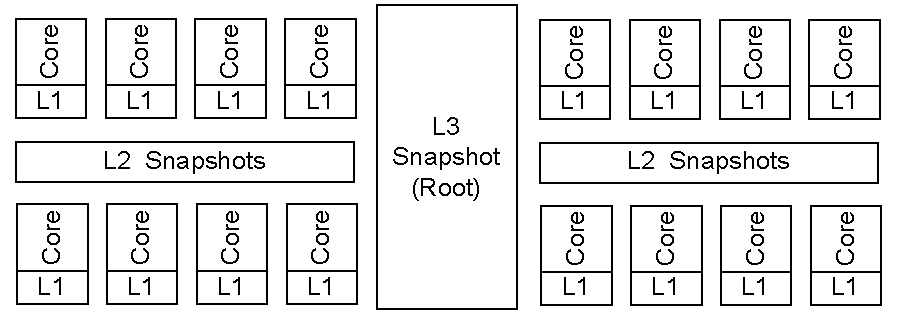
\includegraphics[width=\columnwidth]{images/GFL-mem_layout.drawio.pdf}}
\caption{The architecture of incremental snapshots.}
\vspace{-0.1in}
\label{fig:snapshot}
\end{figure}

\subsection{Reload an Incremental Snapshot}
Once the GPU loads the PTX smart contract via \texttt{cuModuleLoad()}, the global variables will be placed in the data segment. 
We can use \texttt{cuModuleGetGlobal()} to obtain the symbol of the global variable, such as $m$ and $N_i$. 
Next, we query the GPU address of the symbol from  the data table. 
%
Using the GPU address, we can initiate the global storage with designed content in the CPU-end.
%
The GPU address can also help us to export the snapshot data from GPU to the CPU, after each fuzzing iteration.


\subsection{Schedule Incremental Snapshots}
We assume that a vulnerability can be triggered by executing at most two sequential transactions. 
%
To avoid memory latency\cite{bottleneck2015gpu} during transferring incremental snapshots between GPU and CPU, we maintain all snapshots on the GPU memory only. 
%

% To this end, we further design Redirect-On-Write (ROW) snapshot.


\subsection{Coverage Feedback}
Each bitmap uses $2^{16}$ bytes which is designed to handle a smart contract with about $\sqrt{2^{16}} = 256$ basic blocks.
A small bitmap may cause hash collision when computing the bitmap index for an edge. 
To keep flexible, we allow users to configure the bitmap size to meet their requirements. 
%
Since GPUs at most run one warp at the same time, i.e., 32 threads, we declare a global array with 32 bitmaps as $B$.
%
At the end of the code, the PTX code should execute \code{llvm.nvvm.bar.warp.sync} to sync all warp threads.
And then it invokes the runtime function to counter new bits and encodes the results into \texttt{virgin\_bits}. 
To improve the performance, we take a word (8 bytes) each time when traversing the bitmap.


\subsection{Asynchronous GPU Calls}
We create 16 CUDA streams to work together via \texttt{cuStreamCreate()}.
All streams share the same GPU device memory. 
Each stream runs part of threads, where the GPU will allocate a zero-based ID for each thread. 
Thus the threads in different streams should compute their global ID to access the expected memory for data parallelism.
%
For the $l$-th stream, we adjust the thread ID $i$ of its threads to the global one by $i' \gets i + T*l$.
To implement the adjustment, we re-assign the value of $i$ by inserting LLVM IR at the entry of \texttt{@main()}.


\subsection{Sanitizers}
We implement an LLVM Pass as the sanitizer, which accepts LLVM assembly and outputs another LLVM assembly with the sanitizer code.
To be specific, {\tool} supports the following sanitizers. 
\begin{itemize}
    \item \textbf{IntSan} detects integer overflow vulnerabilities. It is inherited from clang's implementation.
    \item \textbf{RenSan} detects reentrancy vulnerabilities. 
\end{itemize}

\subsection{Seed Mutation}
Based on ABI, we design a type-aware mutation engine to mutate the function arguments. 
The mutated seed should also following the function signature.
%
In order to improve the mutation throughput, we did not check the size of function argument in every mutating try. 
To our surprise, every function argument will be serialized into at least one word, i.e., an \texttt{int8} data will also take a word.
According to the types, we use a mask every word to label all type-aware bytes.
For example, \texttt{foo(int8, int32)} has a 2*32 bytes input. We can mutate the input using AFL-favour strategies and then mask with the \texttt{mask = 0xFF << 256 | 0xFFFFFFFF}. Masking is quite cheap, because it only does one AND-operation.
To be specific, {\tool} computes the mask for each target function before the fuzzing. These mask can be reused in the following mutation iteration as the function signature cannot change during the fuzzing. 
This design also benefits {\tool} to reuse AFL code to mutate the bits of seeds. The mirror change is masking with the mutated seeds.
